\documentclass[a4paper, onecolumn, 10pt]{article}

\usepackage[english]{babel}
\usepackage[latin1]{inputenc}
\usepackage[T1]{fontenc}

\usepackage{float} % For controlling figure positions

\usepackage{amsthm} % For using \begin{proof}...
\usepackage{amsfonts}
\usepackage{amssymb}
\usepackage{amsmath}
\usepackage{fancybox}
\usepackage{color}
\usepackage{cite}
\usepackage{url}

\usepackage{algorithm}
\usepackage[noend]{algpseudocode}
\usepackage{program}

\usepackage{authblk}

\title{Neutral competition among prey promotes chaos in two-level food webs\\ {\color{red} Draft}}
\author[1]{Pablo Rodr�guez-S�nchez \thanks{pablo.rodriguezsanchez@wur.nl}}
\author[1]{Egbert van Nes \thanks{egbert.vannes@wur.nl}}
\author[1]{Marten Scheffer \thanks{marten.scheffer@wur.nl}}

\affil[1]{Department of Aquatic Ecology, Wageningen University, The Netherlands}

\usepackage{graphicx}
\graphicspath{ {../img/} }

\usepackage[switch]{lineno}
% TODO: add line numbers and double spacing in the final version
%\linenumbers

\begin{document}

%\title{}
%\author{Pablo Rodr�guez-S�nchez \\ \\ Wageningen University}
%\author{Pablo Rodr�guez-S�nchez \\ \\ pablo.rodriguez.sanchez@gmail.com \\ \\ https://sites.google.com/site/pablorodriguezsanchez/}
%\date{\today}

\maketitle

%\begin{center}
%	\label{fig:QR}
%	\includegraphics[scale=0.4]{QR_main.png}
%\end{center}

\begin{abstract}
\label{sec:Abstract}
Neutral competition can be interpreted as a limit case between dominant intraspecific competition and dominant interspecific competition. Focusing on a numerical model of a two trophic levels ecosystem, the present paper explores the surroundings of this limit case, that is, weak non-neutral competition interactions. It is shown that, the closer the competition is to be neutral, the higher are the chances of the system to develop chaotic behaviour.

% TODO: use more keywords on the abstract and title
\paragraph{}
\textit{Keywords}: population dynamics, competition models, neutral competition, biodiversity paradox, chaos.
\end{abstract}

% TODO: remove/comment in final version
\tableofcontents

\section{Background}
\label{sec:Background} % Introductory paragraph
The fascination by biodiversity is one of the main motivations for studying ecology. Even very young children feel the joy of learning about different species, so no prior knowledge of biology seems to be a requirement for being sensitive to the amazing variety of species. Scientific knowledge increases this sense of wonder even more. Like in a good mystery book, there is a big unknown behind biodiversity: we don't know how it is possible.

\paragraph{} % Introduction of the biodiversity paradox TODO: citations
The mystery comes into scene together with the competitive exclusion principle\cite{Hardin1960}, sometimes referred to as Gause's law. This principle, which some authors trace back to Charles Darwin's \textit{On the origin of the species}\cite{Darwin1859}, is one of the classical touchstones of ecology. The principle states that \textit{"for each niche only one species will dominate in the long run, out-competing the rest"}. Most competition models satisfy this principle, and it has been observed experimentally under laboratory conditions. On the other hand, most of the field observations seem to contradict the competitive exclusion principle, being the huge biodiversity in Earth its most noticeable counterexample. This contradiction is known as the biodiversity paradox. The paradox can be carelessly (but poetically) rephrased as \textit{Why are there so many species?}

%% Brief discussion about the alternative hypotheses
\paragraph{} % Introduction and hypotheses based in non-autonomous systems
There are several alternative hypotheses for escaping the paradox. For instance, Hutchinson\cite{Hutchinson} reports his observations on two sympatric species of beetles competing for the same resource, but not simultaneously because of having different breeding seasons. In a later, influential paper\cite{Hutchinson1961}, Hutchinson proposes the possibility of ecosystems to be driven by external, time-dependent environmental changes. If the characteristic times of this environmental changes are fast enough, the ecosystem is prevented to reach an equilibrium. 

\paragraph{} % Introduction of chaotic dynamics
After the discovery of chaos\cite{Lorenz1963a}, it has been shown that non-equilibrium ecosystems can arise as well under constant environmental conditions\cite{Huisman1999}. More specifically, those ecosystems develop cyclic or chaotic dynamics instead of equilibrium. Of course, chaotic dynamics can arise as well in non-constant environments \cite{Dakos2009b}.

\paragraph{} % Hypotheses based in spatial heterogeneity TODO: enlarge or remove?
All the previous hypotheses refer to the time domain. Regarding the spatial dimension, the inhomogeneity of ecosystems, and the possibility of migration between them has been pointed out as another possible explanation of the paradox \cite{Tilman1994}.

\paragraph{} % Introduction of the neutral theory TODO: citations
Another hypotheses deserving attention are that of neutral competition, whose better known exponent is \textit{Hubbell's neutral competition theory} \cite{Hubbell2001}. In neutral models, similar species inside an ecological community are assumed to have identical per capita rates of birth, rate, reproduction, etc. In those models, the long term differences between species are a result of random events. Despite its counter-intuitive and controversial foundations, neutral models have been successfully applied to populations of rainforest trees.
%% -----

\paragraph{} % Introduction to our contribution TODO: this introduces a bit of a conclusion
In the present paper we show that there is a link between neutral competition and the type of long term dynamics exhibited. Using weakly non-neutral models, our simulations show that the likelihood of chaos increases with neutrality at the competitors' trophic level, having a clear maximum for purely neutral competition. Both neutral hypotheses and the classical non-equilibrium ones seem to not be independent.

\section{Methods}
\label{sec:Methods}

\subsection{Model description}
\label{subsec:Model}
We focused our attention in food webs with two trophic levels, one of consumers and another of prey (see figure \ref{fig:Network}). The consumers predate on the prey, and the prey populations compete among each other for a common resource. These webs are the simplest realization of a system where neutrality doesn't lead to mathematical degeneration (see \ref{sec:Appendix}). Degeneration is prevented by the non-neutral predation rates breaking the excess of symmetry provided by neutrality. % TODO: maybe not needed in an ecology journal

\begin{figure}[h]
	\begin{center}
		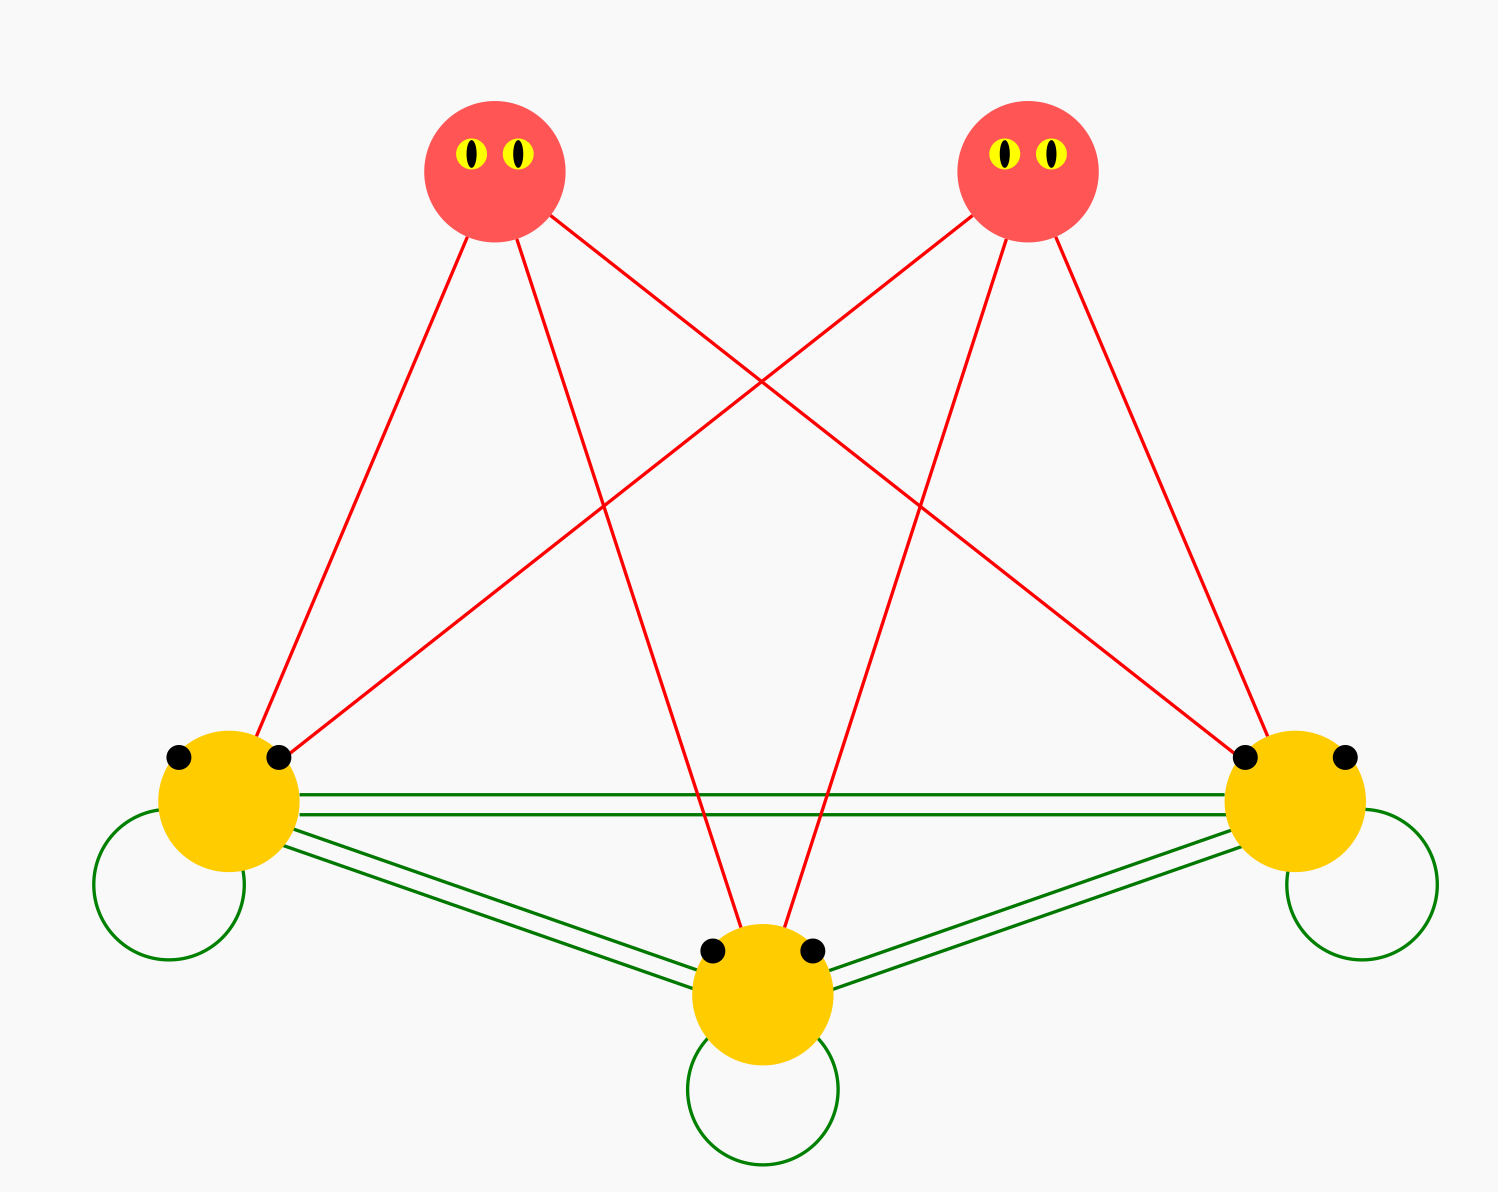
\includegraphics[width=0.7\columnwidth]{net.png}
	\end{center}
	\caption{Example with $2$ consumers and $3$ prey. Each one of the red links represents a predation interaction (coded in the matrix of palatability coefficients, $ S $). Each green link represents a competition interaction (coded in the matrix of competition coefficients, $ A $). The closed green loops are related with carrying capacity (diagonal elements of $ A $) interpreted here as intra-species competition.}
	\label{fig:Network}
\end{figure}

\paragraph{} % Description of the dynamics
The dynamics were modelled as a system of ordinary differential equations. We used a generalized Rosenzweig-MacArthur predator-prey model \cite{Rosenzweig1963, Scheffer2004}, composed of $ n $ prey and $ N $ consumers. $ P_i $ was used for accounting the size of the population of prey $ i $, and $ C_j $ for the population of consumer $ j $. When it is not explicitly stated, $ i $  runs from $ 1 $ to $ n $, and $ j $ from $ 1 $ to $ N $. The prey compete directly among themselves, while the consumers don't interact directly. The prey competition doesn't need to be necessarily symmetrical. The consumers eat all kind of prey (see figure \ref{fig:Network}), but find some of them preferable than others. All these interactions are summarized in \ref{fig:Network}. The overall structure looks like:

\begin{displaymath}
\label{eq:EquationInPseudocode}
	\begin{cases}
	\frac{d}{dt} \left( Prey \right) = Growth  - Predation + Immigration \\
	\frac{d}{dt} \left( Cons \right) = Feeding - Death \\
	\end{cases}
\end{displaymath}

%% Step-by-step description of each term
The growth term is modelled as a multispecies logistic growth. The strength of the competition is given by $ A_{ik} $. Those coefficients can be arranged as a $ n \times n $ matrix. So, for prey $ i $, we have:

\begin{equation}
\label{eq:Growth-Competition}
\resizebox{.8 \columnwidth}{!}
{
$ Growth_i  = r P_i \left( 1 - \frac{1}{K} \sum_{k=1}^n A_{ik} \cdot P_k \right) $
}
\end{equation}

The palatability of each prey species is given by $ S_{ij} $. Those coefficients can be arranged as a $ N \times n $ matrix. Being a multispecies model, we can define the auxiliary variable $ V_j $ as a sum of the prey's populations weighted by the palatability coefficients. Biologically, this represents the composition of the \textit{menu} of consumer $ j $:

\begin{eqnarray}
\label{eq:AuxiliaryVectors}
	V_j \equiv \sum_{k=1}^n S_{jk} \cdot P_k
\end{eqnarray}

We hypothesize that the feeding term will be linear in $ C_j $, and have a Holling type II functional response on $ V_j $ in order to account for consumer satiation:

\begin{equation}
\label{eq:Feeding}
	Feeding_j =  e g C_j F_{2}(V_j; H) = e g C_j \frac{V_j}{V_j + H}
\end{equation}

$ e $ represents the assimilation efficiency of the predation, that is, it regulates the biomass exchange between consumer and prey. Thus, the effect of consumer $ j $ on all prey's populations is given by $ Feeding_j/e $. Knowing this, we can sum the effect of all consumers in the species $ i $ as follows:

\begin{equation}
\label{eq:Predation}
Predation_i = g P_i \sum_{k=1}^N S_{ki} \cdot \frac{C_k}{V_k+H} \equiv gP_iR_i
\end{equation}

Where for convenience, we have defined the auxiliary function $ R_i $ as a summary of this effect of all consumers on prey $ i $:

\begin{equation}
\label{eq:PredationAux}
R_i(C_1, ..., C_N, V_k; S) \equiv \sum_{k=1}^N S_{ki} \cdot \frac{C_k}{V_k+H}
\end{equation}

Putting all together, the dynamical system reads:

\begin{eqnarray}
\label{eq:SystemUnderStudy}
	\begin{cases}
	\dot{P_i} = r P_i \left( 1 - \frac{1}{K} \sum_{k=1}^n A_{ik} \cdot P_k \right) - g P_i R_i + f
	\\ 
	\dot{C_j} = e g C_j \frac{V_j}{V_j + H} - l C_j
	\end{cases}
\end{eqnarray}
%% ------

Depending on the parameters and the initial conditions, this system can give rise to three types of behaviour on the long term, each of them corresponding with a different type of attractor (see figure \ref{fig:TimeSeries}). The easier one, corresponding to a stable point attractor, gives rise to a constant species composition. Cyclic attractors give rise to periodic behaviour in the species composition. Finally, chaotic attractors, make the species composition keep changing without stabilising nor giving rise to periodicity.

% TODO: remove "complex" cyclic attractor
\begin{figure}
	\begin{center}
		\includegraphics[width=.8\columnwidth]{time_series.png}
	\end{center}
	\caption{Time series of the species composition. First figure shows an stable attractor. The second one, a simple cyclic attractor. The third corresponds to a complex cyclic attractor. The last one shows a chaotic attractor}
	\label{fig:TimeSeries}
\end{figure}

\subsection{Parameterization}
\label{subsec:Parameterization}
For the parameterization of our model we used \cite{Dakos2009b} as a reference. Dakos' model, focusing on plankton communities, uses as well a Rosenzweig-McArthur dynamic with two trophic levels (that of zooplankton and phytoplankton). Unlike Dakos, who uses periodic, time-dependent parameters, our parameters will be constant.

\begin{figure}[H]
	\begin{center}
		\resizebox{\columnwidth}{!}{%
		\begin{tabular}{|c|c|c|c|}
			\hline
			\textbf{Symbol} & \textbf{Interpretation} & \textbf{Value} & \textbf{Units} \\
			\hline
			$r$ & Growth rate & $0.5$ & $d^{-1}$ \\
			\hline
			$g$ & Predation rate & $0.4$ & $d^{-1}$\\
			\hline
			$l$ & Loss rate & $0.15$ & $d^{-1}$\\
			\hline
			$K$ & Carrying capacity & $1$ & $ mg \ l^{-1} $ \\
			\hline
			$H$ & Half-saturation constant & $2$ & $ mg \ l^{-1} $\\
			\hline
			$f$ & Immigration rate & $10^{-5}$ & $mg \ l^{-1} \ d^{-1}$\\
		    \hline
			$e$ & Assimilation efficiency & $0.6$ & $1$\\
		    \hline
		    $S$ & $ N \times n $ palatability matrix & $S_{ij} \sim (0,1)$ & $1$\\
		    \hline
   		    $A$ & $ n \times n $ competition matrix & See section \ref{subsec:CompetitionParameter} & $1$\\
		    \hline
		\end{tabular}}
	\end{center}
	\caption{Values and meanings of the parameters used in our numerical experiment}
	\label{tab:Parameters}
\end{figure}

\subsection{Competition parameter}
\label{subsec:CompetitionParameter}

Our aim is to analyse the behaviour of the system described in equation \ref{eq:SystemUnderStudy} for increasingly more neutral competition interactions. But, how can an interaction be more or less neutral? In order to quantify neutrality and controlling the \textit{flavour} of the competition, we introduce the competition parameter $ \epsilon $. This dimensionless parameter will allow us to vary continuously from interactions where intraspecific competition is stronger that interspecific (for $ \epsilon < 0 $) to the opposite case (for $ \epsilon > 0$). The border between both cases (i.e. $ \epsilon = 0 $), where none of the intra non interspecific competition is dominant, represents neutral competition (see figure \ref{tab:CompetitionParameter}). The higher the absolute value of $\epsilon$, the less neutral our model is. 

\paragraph{}
The numerical implementation of these ideas can be easily achieved by building a competition matrix like this:

\begin{eqnarray}
\label{eq:NeutralityParameter}
	A(\epsilon) = A_0 + \epsilon \cdot W
\end{eqnarray}

Where $ A_0 $ is a purely neutral competition matrix (i.e., all its elements equal $ 1 $) and $ W $ is a random matrix whose non-diagonal elements have been drawn from a uniform distribution bounded to the interval $ [0, 1] $, and whose diagonal elements are zero. This way, we make sure that the diagonal elements of $ A $ are $ 1 $ in all cases (see figure \ref{tab:CompetitionParameter}).

\begin{figure}[H]
	\begin{center}
		\resizebox{\columnwidth}{!}{%
		\begin{tabular}{|c|c|c|}
			\hline 
			\textbf{Parameter value} & \textbf{Dominant competition} & \textbf{Example of competition matrix} \\
			\hline 
			$\epsilon < 0$ & Intraspecific & $ A = \begin{bmatrix} 1&.2&.3\\ .3&1&.4 \\ .5&.4&1\end{bmatrix} $ \\ 
			\hline 
			$\epsilon = 0$ & None (neutral) & $A = \begin{bmatrix} 1&1&1\\ 1&1&1 \\ 1&1&1\end{bmatrix}$ \\ 
			\hline 
			$\epsilon > 0$ & Interspecific & $A = \begin{bmatrix} 1&1.7&1.6\\ 1.9&1&1.5 \\ 1.8&1.6&1\end{bmatrix}$ \\ 
			\hline 
		\end{tabular}}
	\end{center}
	\caption{Effect of the competition parameter on the competition matrix}	
	\label{tab:CompetitionParameter}
\end{figure}

% TODO: maybe to appendix?
\subsection{Detection of chaos}
\label{subsec:DetectionOfChaos}
Dynamical systems with chaotic attractors are extremelly sensitive to initial conditions. Two trajectories whose initial conditions are slightly different will diverge exponentially if they lie in the basin of a chaotic attractor. The rate of divergence is quantified by the Lyapunov exponent \cite{Strogatz1994}.

\paragraph{}
Our procedure for classifying the attractors as chaotic or non-chaotic was based in the analysis of Lyapunov exponents. More specifically, this is the procedure we've followed:

\begin{enumerate}
	\item \label{GoToAttractor} Run the simulation for time enough, in order to guarantee that an attractor has been reached
	\item \label{RunInAttractor} Use the run in step \ref{GoToAttractor} as a starting point for a second, shorter run inside the attractor
	\item Use the run in step \ref{RunInAttractor} to compute numerically the principal Lyapunov exponent	
	\begin{itemize}
		\item If it's positive, classify the attractor as chaotic
		\item If it's negative, classify the attractor as non-chaotic
	\end{itemize}
\end{enumerate}

{\color{red} Big warning here: our method for detecting chaos sometimes gives false positives for complex cycles}

\subsection{Numerical experiment}
\label{subsec:NumericalExperiment}
Our main target is to estimate the probability of a chaotic attractor under different intensities of neutrality. Due to the complexity of the system, we face the problem as a numerical simulation\footnote{The present analysis were performed using GRIND for MATLAB. It's freely available at \\ \url{http://www.sparcs-center.org/grind.html}}. As well, and for the sake of reproducibility, we provide a \textit{GitHub} link to the scripts used. {\color{red}Discuss with Egbert and Marten about which code repository use}

\paragraph{}
Sweeping for different values of $ \epsilon $, we use the following procedure to estimate the probability of a chaotic attractor:

\begin{enumerate}
	\item Use the competition parameter $\epsilon$ to draw a competition matrix $A$ (as described in section \ref{subsec:CompetitionParameter}). Notice that this matrix will change in every run
	\item \label{StartOfAnExperiment} Draw the rest of parameters and initial conditions from the ranges described in \cite{Dakos2009b}, taken as uniform PDFs. Notice that those parameters taken from a PDF will change in every run
	\item Determine numerically if the attractor generated by this conditions is chaotic or not (see section \ref{subsec:DetectionOfChaos})
	\item Go back to step (\ref{StartOfAnExperiment}) $R$ times
\end{enumerate}

For those more familiar with flow charts, figure \ref{fig:FlowChart} can be illuminating.

\begin{figure}[H]
	\begin{center}
		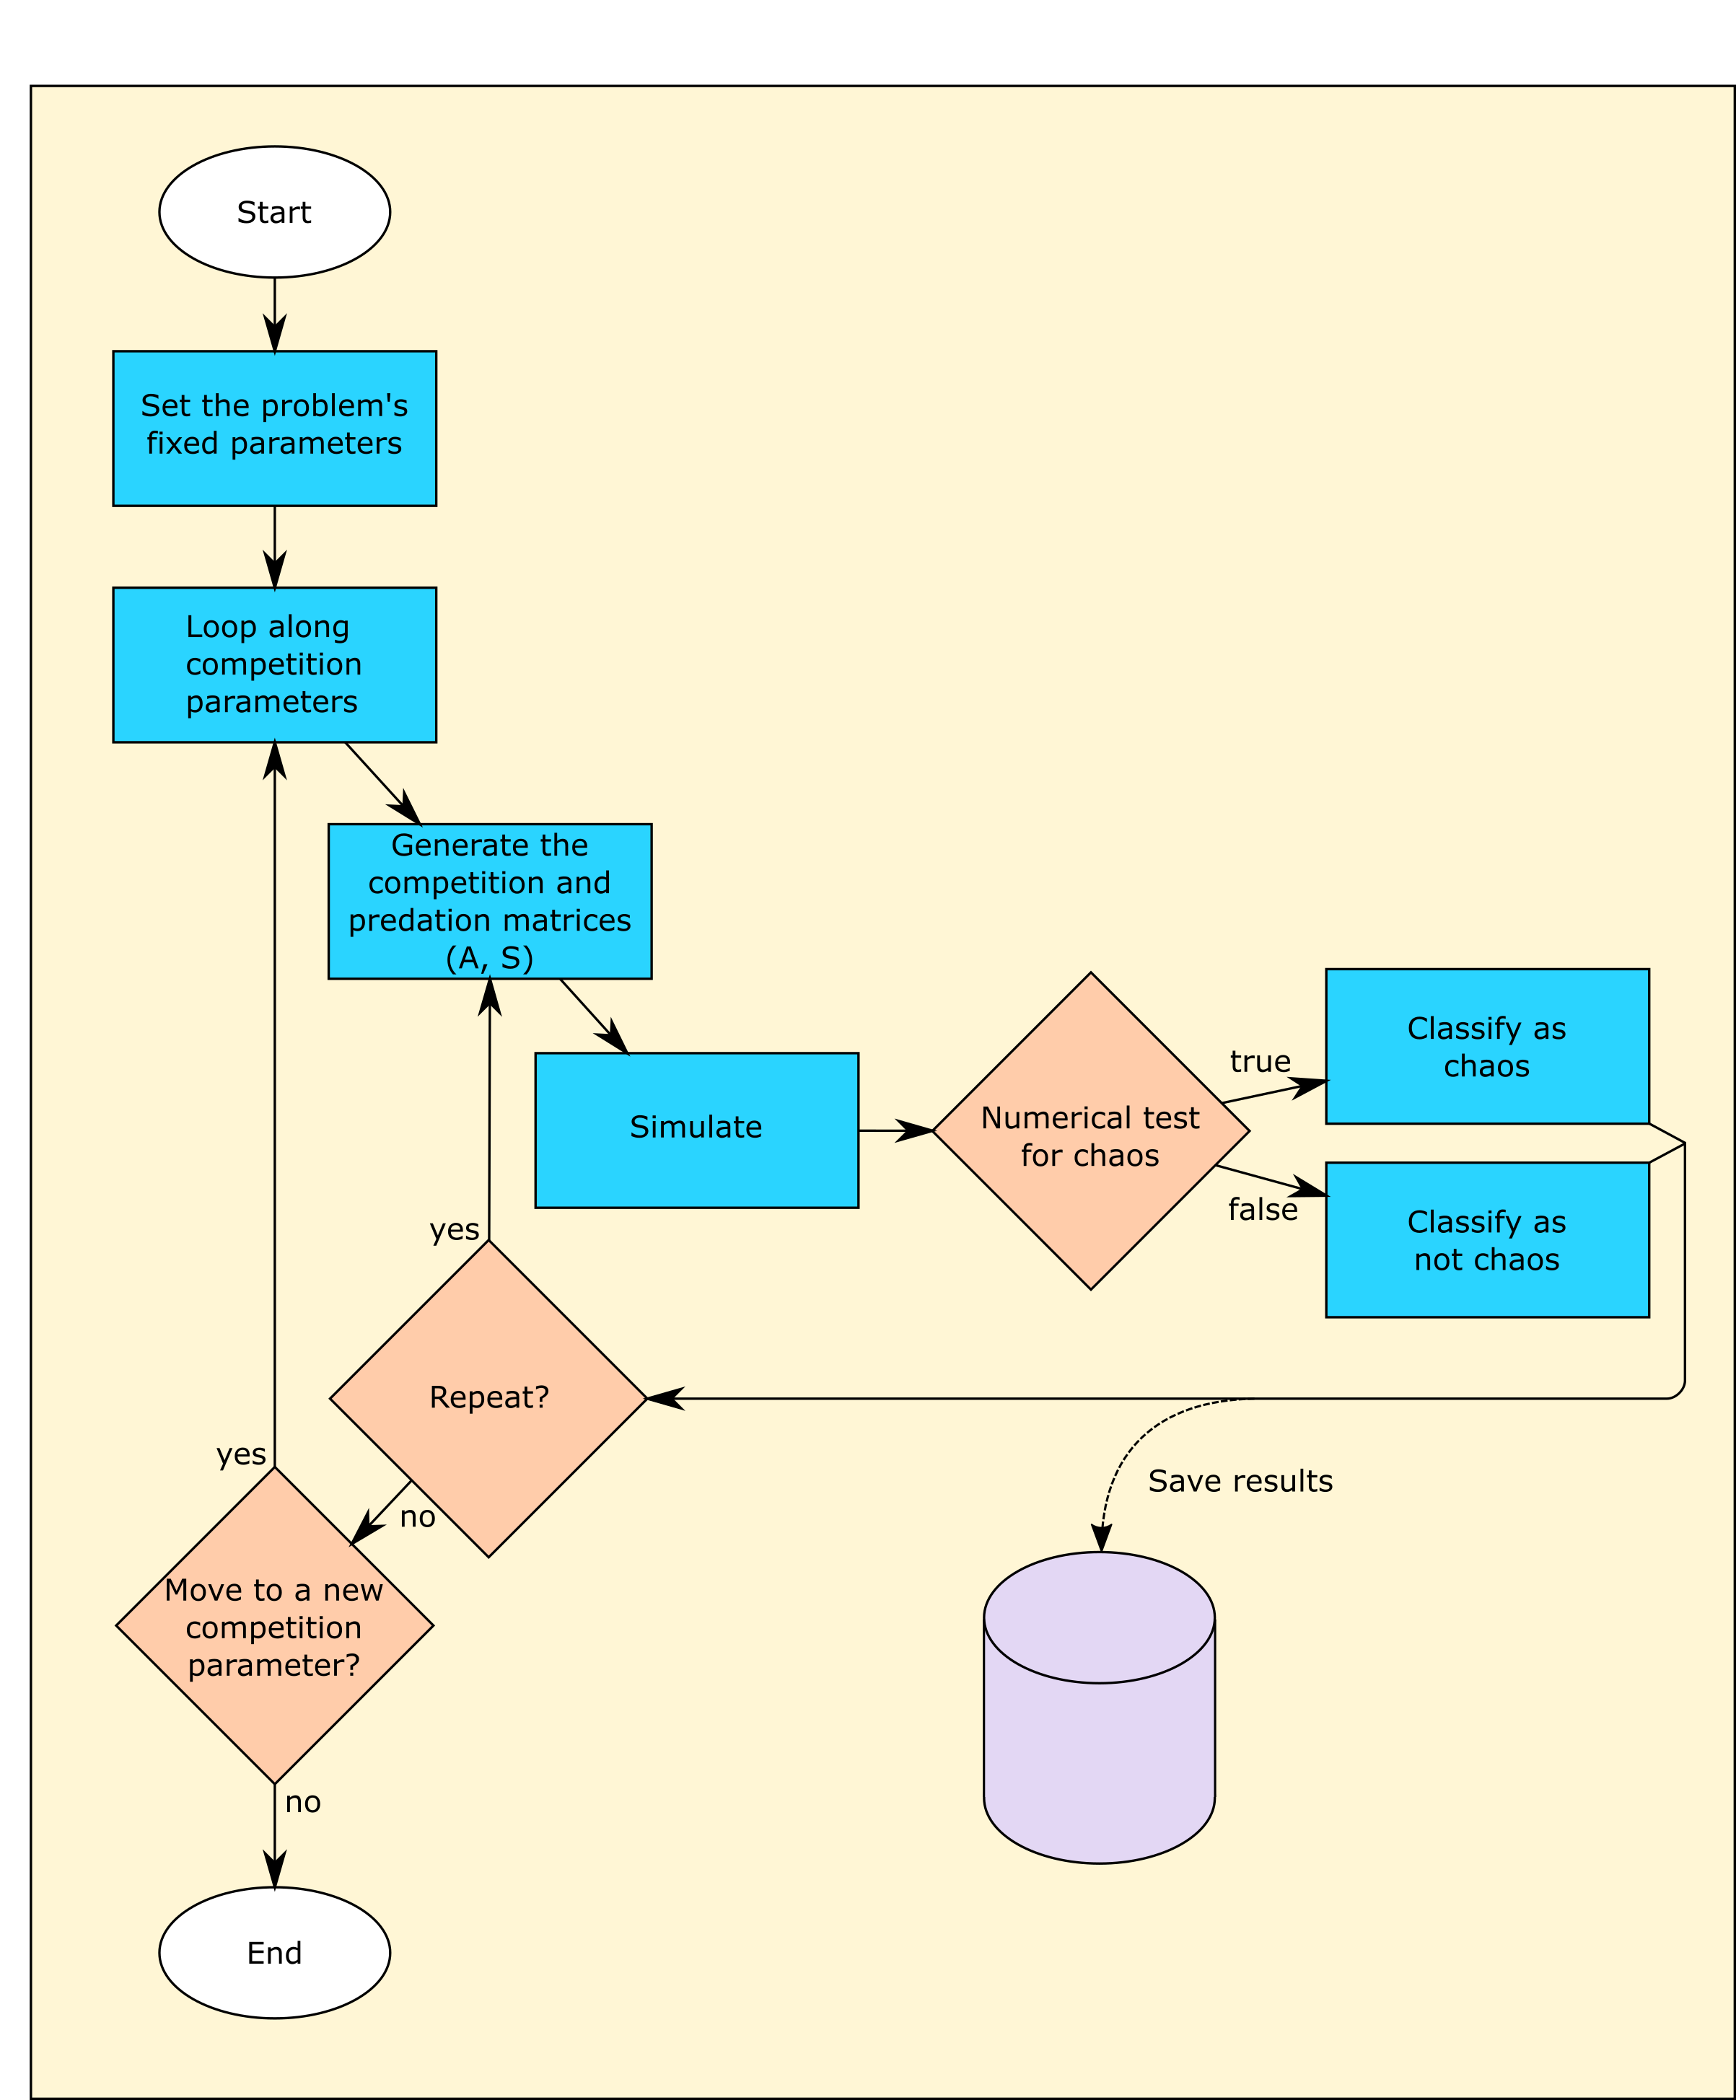
\includegraphics[width=0.9\columnwidth]{flow_chart.png}
	\end{center}
	\caption{Flow chart describing the numerical experiment}
	\label{fig:FlowChart}
\end{figure}

The outcome of the numerical experiment described above is a list of $ R $ maximum Lyapunov exponents per value of $ \epsilon $. This list can be used to estimate the probability of chaos for each value of $ \epsilon $ via the classical frequentist interpretation of probability, that is, as the ratio of attractors found to be chaotic.

% TODO: maybe remove?
\begin{equation}
\label{eq:Probability}
	P(Chaos) \approx \frac{\#_{chaos}}{\#_{total}}
\end{equation}

\paragraph*{}
This numerical experiment can be repeated for food webs of different sizes. In our simulations, we kept a ratio of 2:3 for the number of species at the consumer and the prey level.

\section{Results}
\label{sec:Results}

Plotting the probability of chaos against the competition parameter (see figures \ref{fig:Results} and \ref{fig:Contour}), we observe a clear maximum around $ \epsilon = 0 $. That is, for neutral competition at the prey's trophic level, the likelihood of chaotic behaviour is higher than for dominant inter or intraspecific competition. From the biological point of view, we show that neutrality and non-equilibrium dynamics are not completely independent. Maybe this can be a first step to reconcile both views.

\paragraph{} % Weak and strong interspecific competition
The probability of chaos when intraspecific competition is dominant has a valley between $ \epsilon = -1 $ and $ \epsilon = 0 $. We interpret this result as the overlap of two effects. On the one hand, as we have shown, weak dominant interspecific competition is less prone to chaos than neutral competition. On the other, strong interspecific competition increases the likelihood of chaos again. Assuming continuity, there has to be necessarily at least one minimum between both cases by virtue of Rolle's theorem \cite{Simmons1996}.
% TODO: increase even more the range of the parameter?

\paragraph{} % Chaos and dimensionality
The overall likelihood of chaos increases with the size of the food web. This effect should not be surprising: the more dimensions the phase space has, the easier is to develop the complex geometry of a chaotic attractor. Intuitively, we can understand this as increasing the available room for the formation of the attractor. Even in those higher dimensional cases, a maximum is still happening at the neutral competition case.

\begin{figure}
	\begin{center}
		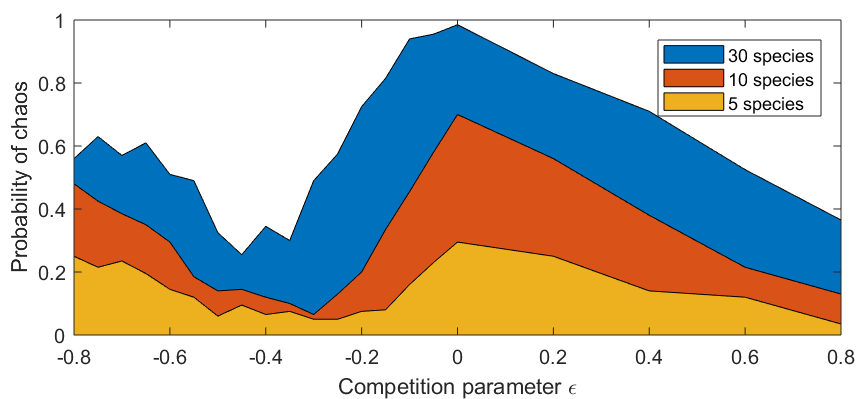
\includegraphics[width=0.9\columnwidth]{results.png}
	\end{center}
	\caption{Results for a low, medium and high dimensional system. The upper row represents the measured Lyapunov exponents, coloured in red if larger than zero, and in blue if lower. The lower row represents the estimated probability of chaotic behaviour}
	\label{fig:Results}
\end{figure}

\begin{figure}
	\begin{center}
		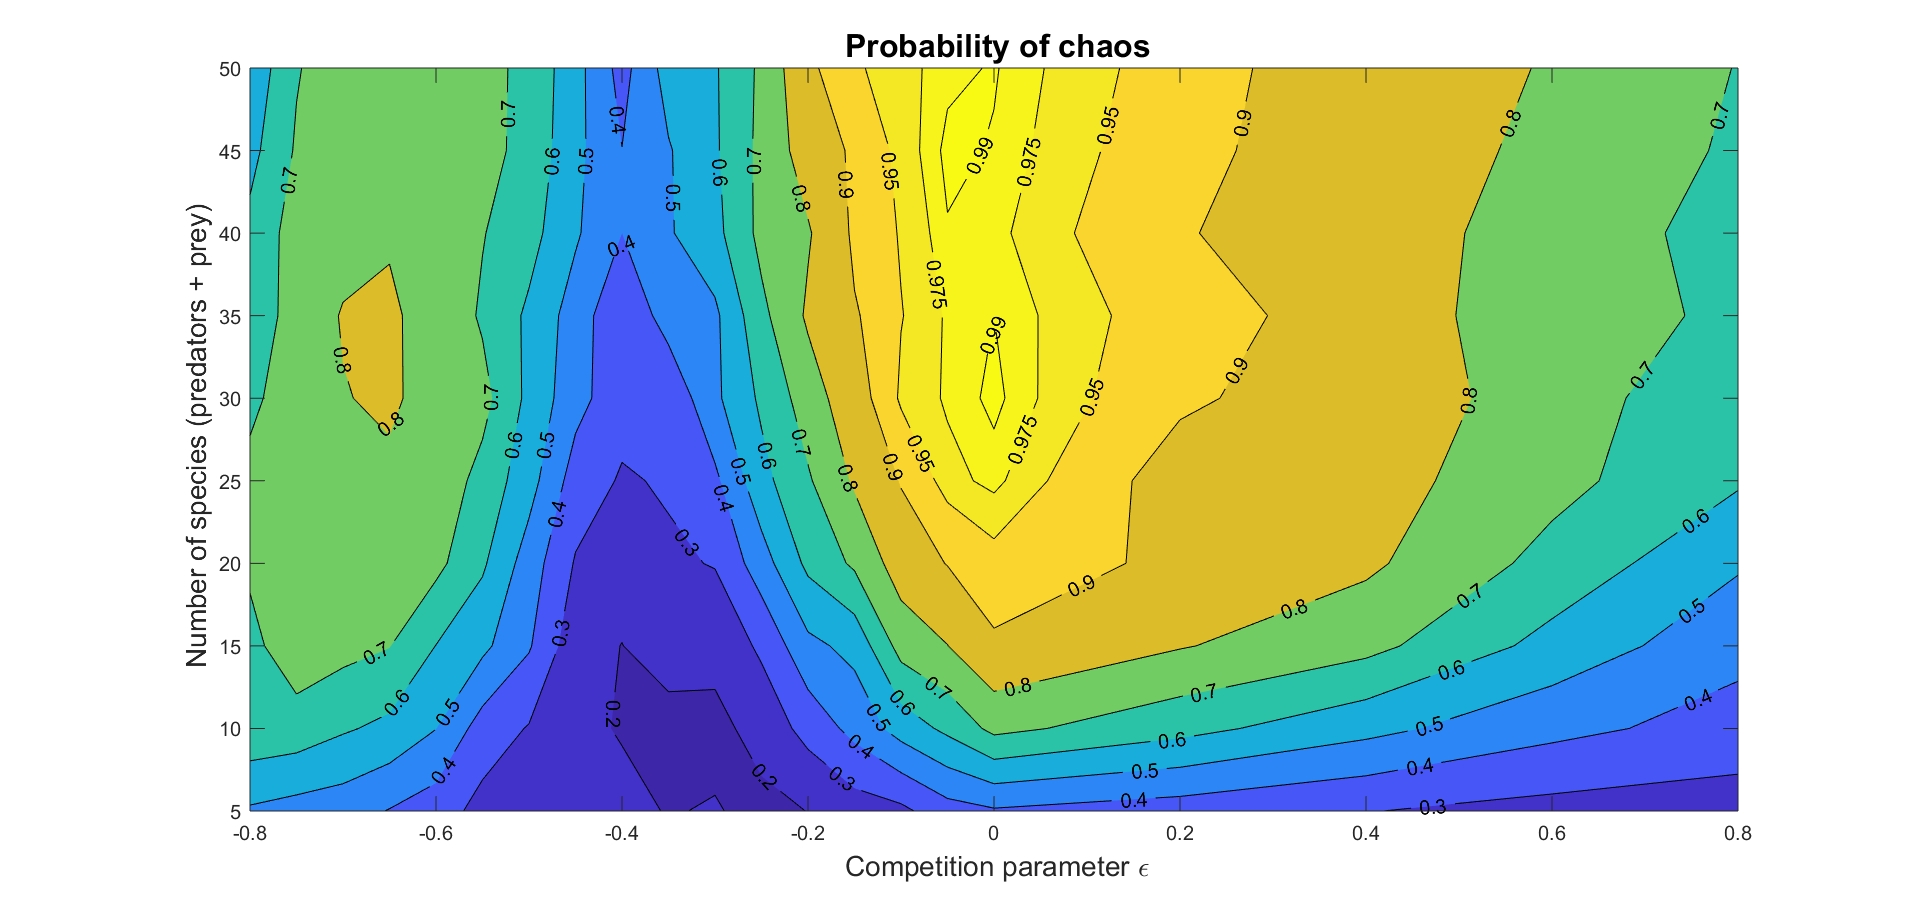
\includegraphics[width=1\columnwidth]{contour.png}
	\end{center}
	\caption{Contour map showing the probability of chaos for various competition parameters (horizontal axis) and prey populations (vertical axis). The consumers' population is fixed as $ 2/3 $ of the prey's population, in order to control the overall size of the system with a single parameter. Notice that chaotic attractors appear more easily (i.e., for smaller systems) if the competition is neutral (i.e., $ \epsilon = 0 $)}
	\label{fig:Contour}
\end{figure}

% TODO: use conclusions and discussion. What's the difference?
\section{Conclusions}
\label{sec:Conclusions}

\section{Appendix}
\label{sec:Appendix}

\subsection{Neutral competition}
\label{subsec:NeutralCompetition}
If we drop everything but the competition part of our dynamics (see equation \ref{eq:SystemUnderStudy}), we will find a system of equations $ n $ like the following:

\begin{eqnarray}
\label{eq:OnlyCompetition}
\dot{P_i} = P_i \left( 1 - \sum_{k=1}^n A_{ik} \cdot P_k \right)
\end{eqnarray}

In order to model a neutral competition, we should use the same competition coefficient for each species. That is, take $ A_{ik} = A $ for all $ i $ and $ k $, so:

\begin{eqnarray}
\label{eq:OnlyNeutralCompetition}
\dot{P_i} = P_i \left( 1 - A \sum_{k=1}^n P_k \right)
\end{eqnarray}

From equation \ref{eq:OnlyNeutralCompetition} we see that all species have exactly the same dynamical equation. This will make the nullclines to coincide at all points, so the equilibrium points will degenerate to equilibrium manifolds.

\begin{figure}[h]
	\begin{center}
		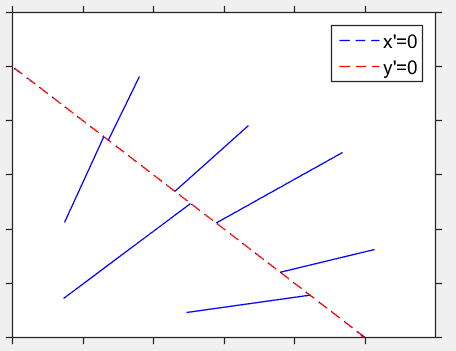
\includegraphics[width=0.9\columnwidth]{degenerate.png}
	\end{center}
	\caption{Example with $2$ prey under neutral competition. Both nullclines coincide point to point, giving rise to a higher dimensional equilibirium manifold (in this case, a straight line)}
	\label{fig:Neutral}
\end{figure}

This problem can be solved more easily noticing that, from the sole point of view of competition, the effect of neutrality is to fade out the differences between species. Being this the case, the labels $ i $ distinguishing them become pointless. It is a good idea to sum up all the competing species into a new variable, that of total population of (now indistinguishable) species, defined by:

\begin{eqnarray}
\label{eq:TotalPopulation}
	T(t) = \sum_{i=1}^n P_i(t)
\end{eqnarray}

It can be shown using equation \ref{eq:OnlyNeutralCompetition} that, as expected from the biological intuition, the dynamics of this new variable will follow the same differential equation as the individual species abundances. This collapses the $ n $ dimensions of our original problem to a single one.

\begin{eqnarray}
\label{eq:TotalPopulationDynamics}
	\dot T(t) = \sum_{i=1}^n \dot P_i(t) = T (1 - A T)
\end{eqnarray}

In our model, the predation interaction breaks this excess of symmetry, so we can still work with neutral competition as long as the predation is not neutral without facing problems of system degeneration.


\section{Acknowledgements}
\label{sec:Acknowledgements}
We thank Jelle Lever, for his useful comments and suggestions.

\color{red}
\section{To do}
\label{sec:ToDo}

\begin{itemize}
\item Send more details to the appendix?
\item Remove or improve the pseudocode algorithm
\item Clean and publish analysis code in \textit{GitHub}
\end{itemize}

Further ideas, for this or future papers:

\begin{itemize}
\item Neutrality in predation
\item Study symmetric competition with a parameter that controls symmetry
\item Neutrality increases symmetry as well. May this be related with the fact that, as said in \cite{Scheffer2004}, \textit{"symmetry in competition strongly promotes multiplicity of attractors"}
\end{itemize}


\color{black}
\clearpage

% TODO: format citations
\bibliography{library}
\bibliographystyle{ieeetr}
%\bibliographystyle{apalike}

%\listoftables
\listoffigures

\end{document}

%% Notes
%
% Are there better names for "dominant interspecific competition"?
% Focus on two hypotheses
% Describe every term in the equations?